\documentclass[../tex_main/NEMO_manual]{subfiles}
\begin{document}
% ================================================================
% Chapter —— Surface Boundary Condition (SBC, ISF, ICB) 
% ================================================================
\chapter{Surface Boundary Condition (SBC, ISF, ICB) }
\label{chap:SBC}
\minitoc

\newpage
$\ $\newline    % force a new ligne
%---------------------------------------namsbc--------------------------------------------------

\nlst{namsbc}
%--------------------------------------------------------------------------------------------------------------
$\ $\newline    % force a new ligne

The ocean needs six fields as surface boundary condition:
\begin{itemize}
\item
  the two components of the surface ocean stress $\left( {\tau _u \;,\;\tau _v} \right)$
\item
  the incoming solar and non solar heat fluxes $\left( {Q_{ns} \;,\;Q_{sr} } \right)$
\item
  the surface freshwater budget $\left( {\textit{emp}} \right)$
\item
  the surface salt flux associated with freezing/melting of seawater $\left( {\textit{sfx}} \right)$
\end{itemize}
plus an optional field:
\begin{itemize}
	\item the atmospheric pressure at the ocean surface $\left( p_a \right)$
\end{itemize}

Four different ways to provide the first six fields to the ocean are available which are controlled by
namelist \ngn{namsbc} variables:
an analytical formulation (\np{ln\_ana}\forcode{ = .true.}),
a flux formulation (\np{ln\_flx}\forcode{ = .true.}),
a bulk formulae formulation (CORE (\np{ln\_blk\_core}\forcode{ = .true.}),
CLIO (\np{ln\_blk\_clio}\forcode{ = .true.}) bulk formulae) and
a coupled or mixed forced/coupled formulation (exchanges with a atmospheric model via the OASIS coupler)
(\np{ln\_cpl} or \np{ln\_mixcpl}\forcode{ = .true.}). 
When used ($i.e.$ \np{ln\_apr\_dyn}\forcode{ = .true.}),
the atmospheric pressure forces both ocean and ice dynamics.

The frequency at which the forcing fields have to be updated is given by the \np{nn\_fsbc} namelist parameter.
When the fields are supplied from data files (flux and bulk formulations),
the input fields need not be supplied on the model grid.
Instead a file of coordinates and weights can be supplied which maps the data from the supplied grid to
the model points (so called "Interpolation on the Fly", see \autoref{subsec:SBC_iof}).
If the Interpolation on the Fly option is used, input data belonging to land points (in the native grid),
can be masked to avoid spurious results in proximity of the coasts as
large sea-land gradients characterize most of the atmospheric variables.

In addition, the resulting fields can be further modified using several namelist options.
These options control 
\begin{itemize}
\item
  the rotation of vector components supplied relative to an east-north coordinate system onto
  the local grid directions in the model;
\item
  the addition of a surface restoring term to observed SST and/or SSS (\np{ln\_ssr}\forcode{ = .true.});
\item
  the modification of fluxes below ice-covered areas (using observed ice-cover or a sea-ice model)
  (\np{nn\_ice}\forcode{ = 0..3});
\item
  the addition of river runoffs as surface freshwater fluxes or lateral inflow (\np{ln\_rnf}\forcode{ = .true.});
\item
  the addition of isf melting as lateral inflow (parameterisation) or
  as fluxes applied at the land-ice ocean interface (\np{ln\_isf}) ; 
\item
  the addition of a freshwater flux adjustment in order to avoid a mean sea-level drift
  (\np{nn\_fwb}\forcode{ = 0..2});
\item
  the transformation of the solar radiation (if provided as daily mean) into a diurnal cycle
  (\np{ln\_dm2dc}\forcode{ = .true.});
\item
  a neutral drag coefficient can be read from an external wave model (\np{ln\_cdgw}\forcode{ = .true.});
\item
  the Stokes drift rom an external wave model can be accounted (\np{ln\_sdw}\forcode{ = .true.}); 
\item
  the Stokes-Coriolis term can be included (\np{ln\_stcor}\forcode{ = .true.});
\item
  the surface stress felt by the ocean can be modified by surface waves (\np{ln\_tauwoc}\forcode{ = .true.}).
\end{itemize}

In this chapter, we first discuss where the surface boundary condition appears in the model equations.
Then we present the five ways of providing the surface boundary condition, 
followed by the description of the atmospheric pressure and the river runoff. 
Next the scheme for interpolation on the fly is described.
Finally, the different options that further modify the fluxes applied to the ocean are discussed.
One of these is modification by icebergs (see \autoref{sec:ICB_icebergs}),
which act as drifting sources of fresh water.
Another example of modification is that due to the ice shelf melting/freezing (see \autoref{sec:SBC_isf}), 
which provides additional sources of fresh water.


% ================================================================
% Surface boundary condition for the ocean
% ================================================================
\section{Surface boundary condition for the ocean}
\label{sec:SBC_general}

The surface ocean stress is the stress exerted by the wind and the sea-ice on the ocean.
It is applied in \mdl{dynzdf} module as a surface boundary condition of the computation of
the momentum vertical mixing trend (see \autoref{eq:dynzdf_sbc} in \autoref{sec:DYN_zdf}).
As such, it has to be provided as a 2D vector interpolated onto the horizontal velocity ocean mesh,
$i.e.$ resolved onto the model (\textbf{i},\textbf{j}) direction at $u$- and $v$-points.

The surface heat flux is decomposed into two parts, a non solar and a solar heat flux,
$Q_{ns}$ and $Q_{sr}$, respectively.
The former is the non penetrative part of the heat flux
($i.e.$ the sum of sensible, latent and long wave heat fluxes plus
the heat content of the mass exchange with the atmosphere and sea-ice).
It is applied in \mdl{trasbc} module as a surface boundary condition trend of
the first level temperature time evolution equation
(see \autoref{eq:tra_sbc} and \autoref{eq:tra_sbc_lin} in \autoref{subsec:TRA_sbc}). 
The latter is the penetrative part of the heat flux.
It is applied as a 3D trends of the temperature equation (\mdl{traqsr} module) when
\np{ln\_traqsr}\forcode{ = .true.}.
The way the light penetrates inside the water column is generally a sum of decreasing exponentials
(see \autoref{subsec:TRA_qsr}). 

The surface freshwater budget is provided by the \textit{emp} field.
It represents the mass flux exchanged with the atmosphere (evaporation minus precipitation) and
possibly with the sea-ice and ice shelves (freezing minus melting of ice).
It affects both the ocean in two different ways:
$(i)$  it changes the volume of the ocean and therefore appears in the sea surface height equation as
a volume flux, and 
$(ii)$ it changes the surface temperature and salinity through the heat and salt contents of
the mass exchanged with the atmosphere, the sea-ice and the ice shelves. 


%\colorbox{yellow}{Miss: }
%
%A extensive description of all namsbc namelist (parameter that have to be 
%created!)
%
%Especially the \np{nn\_fsbc}, the \mdl{sbc\_oce} module (fluxes + mean sst sss ssu 
%ssv) i.e. information required by flux computation or sea-ice
%
%\mdl{sbc\_oce} containt the definition in memory of the 7 fields (6+runoff), add 
%a word on runoff: included in surface bc or add as lateral obc{\ldots}.
%
%Sbcmod manage the ``providing'' (fourniture) to the ocean the 7 fields
%
%Fluxes update only each nf{\_}sbc time step (namsbc) explain relation 
%between nf{\_}sbc and nf{\_}ice, do we define nf{\_}blk??? ? only one 
%nf{\_}sbc
%
%Explain here all the namlist namsbc variable{\ldots}.
% 
% explain : use or not of surface currents
%
%\colorbox{yellow}{End Miss }

The ocean model provides, at each time step, to the surface module (\mdl{sbcmod})
the surface currents, temperature and salinity.  
These variables are averaged over \np{nn\_fsbc} time-step (\autoref{tab:ssm}), and
it is these averaged fields which are used to computes the surface fluxes at a frequency of \np{nn\_fsbc} time-step.


%-------------------------------------------------TABLE---------------------------------------------------
\begin{table}[tb]   \begin{center}   \begin{tabular}{|l|l|l|l|}
\hline
Variable description					& Model variable	& Units	& point \\	\hline
i-component of the surface current	& ssu\_m	& $m.s^{-1}$	& U \\	\hline
j-component of the surface current	& ssv\_m	& $m.s^{-1}$	& V \\	\hline
Sea surface temperature				& sst\_m	& \r{}$K$		& T \\	\hline
Sea surface salinty					& sss\_m	& $psu$			& T \\	\hline
\end{tabular}
\caption{  \protect\label{tab:ssm}
  Ocean variables provided by the ocean to the surface module (SBC).
  The variable are averaged over nn{\_}fsbc time step,
  $i.e.$ the frequency of computation of surface fluxes.}
\end{center}   \end{table}
%--------------------------------------------------------------------------------------------------------------

%\colorbox{yellow}{Penser a} mettre dans le restant l'info nn{\_}fsbc ET nn{\_}fsbc*rdt de sorte de reinitialiser la moyenne si on change la frequence ou le pdt


% ================================================================
%       Input Data 
% ================================================================
\section{Input data generic interface}
\label{sec:SBC_input}

A generic interface has been introduced to manage the way input data
(2D or 3D fields, like surface forcing or ocean T and S) are specify in \NEMO.
This task is archieved by \mdl{fldread}.
The module was design with four main objectives in mind: 
\begin{enumerate}
\item
  optionally provide a time interpolation of the input data at model time-step, whatever their input frequency is,
  and according to the different calendars available in the model.
\item
  optionally provide an on-the-fly space interpolation from the native input data grid to the model grid.
\item
  make the run duration independent from the period cover by the input files.
\item
  provide a simple user interface and a rather simple developer interface by
  limiting the number of prerequisite information. 
\end{enumerate}  

As a results the user have only to fill in for each variable a structure in the namelist file to
define the input data file and variable names, the frequency of the data (in hours or months),
whether its is climatological data or not, the period covered by the input file (one year, month, week or day),
and three additional parameters for on-the-fly interpolation.
When adding a new input variable, the developer has to add the associated structure in the namelist,
read this information by mirroring the namelist read in \rou{sbc\_blk\_init} for example,
and simply call \rou{fld\_read} to obtain the desired input field at the model time-step and grid points.

The only constraints are that the input file is a NetCDF file, the file name follows a nomenclature 
(see \autoref{subsec:SBC_fldread}), the period it cover is one year, month, week or day, and,
if on-the-fly interpolation is used, a file of weights must be supplied (see \autoref{subsec:SBC_iof}).

Note that when an input data is archived on a disc which is accessible directly from the workspace where
the code is executed, then the use can set the \np{cn\_dir} to the pathway leading to the data.
By default, the data are assumed to have been copied so that cn\_dir='./'.

% -------------------------------------------------------------------------------------------------------------
% Input Data specification (\mdl{fldread})
% -------------------------------------------------------------------------------------------------------------
\subsection{Input data specification (\protect\mdl{fldread})}
\label{subsec:SBC_fldread}

The structure associated with an input variable contains the following information:
\begin{forlines}
!  file name  ! frequency (hours) ! variable  ! time interp. !  clim  ! 'yearly'/ ! weights  ! rotation ! land/sea mask ! 
!             !  (if <0  months)  !   name    !   (logical)  !  (T/F) ! 'monthly' ! filename ! pairing  ! filename      !
\end{forlines}
where 
\begin{description}  
\item[File name]:
  the stem name of the NetCDF file to be open.
  This stem will be completed automatically by the model, with the addition of a '.nc' at its end and
  by date information and possibly a prefix (when using AGRIF).
  Tab.\autoref{tab:fldread} provides the resulting file name in all possible cases according to
  whether it is a climatological file or not, and to the open/close frequency (see below for definition).

%--------------------------------------------------TABLE--------------------------------------------------
\begin{table}[htbp] 
\begin{center}
\begin{tabular}{|l|c|c|c|}
\hline
                         & daily or weekLLL	        & monthly                   &   yearly          \\   \hline
\np{clim}\forcode{ = .false.}	& fn\_yYYYYmMMdDD.nc  &   fn\_yYYYYmMM.nc   &   fn\_yYYYY.nc  \\   \hline
\np{clim}\forcode{ = .true.}	 	   & not possible 	              &  fn\_m??.nc             &   fn                \\   \hline
\end{tabular}
\end{center}
\caption{ \protect\label{tab:fldread}
  naming nomenclature for climatological or interannual input file, as a function of the Open/close frequency.
  The stem name is assumed to be 'fn'.
  For weekly files, the 'LLL' corresponds to the first three letters of the first day of the week
  ($i.e.$ 'sun','sat','fri','thu','wed','tue','mon').
  The 'YYYY', 'MM' and 'DD' should be replaced by the actual year/month/day, always coded with 4 or 2 digits.
  Note that (1) in mpp, if the file is split over each subdomain, the suffix '.nc' is replaced by '\_PPPP.nc',
  where 'PPPP' is the process number coded with 4 digits;
  (2) when using AGRIF, the prefix '\_N' is added to files, where 'N'  is the child grid number.}
\end{table}
%--------------------------------------------------------------------------------------------------------------
  

\item[Record frequency]:
  the frequency of the records contained in the input file.
  Its unit is in hours if it is positive (for example 24 for daily forcing) or in months if negative
  (for example -1 for monthly forcing or -12 for annual forcing).
  Note that this frequency must really be an integer and not a real.
  On some computers, seting it to '24.' can be interpreted as 240!

\item[Variable name]:
  the name of the variable to be read in the input NetCDF file.

\item[Time interpolation]:
  a logical to activate, or not, the time interpolation.
  If set to 'false', the forcing will have a steplike shape remaining constant during each forcing period.
  For example, when using a daily forcing without time interpolation, the forcing remaining constant from
  00h00'00'' to 23h59'59".
  If set to 'true', the forcing will have a broken line shape.
  Records are assumed to be dated the middle of the forcing period.
  For example, when using a daily forcing with time interpolation,
  linear interpolation will be performed between mid-day of two consecutive days. 

\item[Climatological forcing]:
  a logical to specify if a input file contains climatological forcing which can be cycle in time,
  or an interannual forcing which will requires additional files if
  the period covered by the simulation exceed the one of the file.
  See the above the file naming strategy which impacts the expected name of the file to be opened. 

\item[Open/close frequency]:
  the frequency at which forcing files must be opened/closed.
  Four cases are coded:
  'daily', 'weekLLL' (with 'LLL' the first 3 letters of the first day of the week), 'monthly' and 'yearly' which
  means the forcing files will contain data for one day, one week, one month or one year.
  Files are assumed to contain data from the beginning of the open/close period.
  For example, the first record of a yearly file containing daily data is Jan 1st even if
  the experiment is not starting at the beginning of the year. 

\item[Others]:
  'weights filename', 'pairing rotation' and 'land/sea mask' are associated with
  on-the-fly interpolation which is described in \autoref{subsec:SBC_iof}.

\end{description}

Additional remarks:\\
(1) The time interpolation is a simple linear interpolation between two consecutive records of the input data.
The only tricky point is therefore to specify the date at which we need to do the interpolation and
the date of the records read in the input files.
Following \citet{Leclair_Madec_OM09}, the date of a time step is set at the middle of the time step.
For example, for an experiment starting at 0h00'00" with a one hour time-step,
a time interpolation will be performed at the following time: 0h30'00", 1h30'00", 2h30'00", etc.
However, for forcing data related to the surface module,
values are not needed at every time-step but at every \np{nn\_fsbc} time-step.
For example with \np{nn\_fsbc}\forcode{ = 3}, the surface module will be called at time-steps 1, 4, 7, etc.
The date used for the time interpolation is thus redefined to be at the middle of \np{nn\_fsbc} time-step period.
In the previous example, this leads to: 1h30'00", 4h30'00", 7h30'00", etc. \\ 
(2) For code readablility and maintenance issues, we don't take into account the NetCDF input file calendar.
The calendar associated with the forcing field is build according to the information provided by
user in the record frequency, the open/close frequency and the type of temporal interpolation.
For example, the first record of a yearly file containing daily data that will be interpolated in time is assumed to
be start Jan 1st at 12h00'00" and end Dec 31st at 12h00'00". \\
(3) If a time interpolation is requested, the code will pick up the needed data in the previous (next) file when
interpolating data with the first (last) record of the open/close period.
For example, if the input file specifications are ''yearly, containing daily data to be interpolated in time'', 
the values given by the code between 00h00'00" and 11h59'59" on Jan 1st will be interpolated values between
Dec 31st 12h00'00" and Jan 1st 12h00'00".
If the forcing is climatological, Dec and Jan will be keep-up from the same year.
However, if the forcing is not climatological, at the end of
the open/close period the code will automatically close the current file and open the next one.
Note that, if the experiment is starting (ending) at the beginning (end) of
an open/close period we do accept that the previous (next) file is not existing.
In this case, the time interpolation will be performed between two identical values.
For example, when starting an experiment on Jan 1st of year Y with yearly files and daily data to be interpolated,
we do accept that the file related to year Y-1 is not existing.
The value of Jan 1st will be used as the missing one for Dec 31st of year Y-1.
If the file of year Y-1 exists, the code will read its last record. 
Therefore, this file can contain only one record corresponding to Dec 31st,
a useful feature for user considering that it is too heavy to manipulate the complete file for year Y-1.


% -------------------------------------------------------------------------------------------------------------
% Interpolation on the Fly
% -------------------------------------------------------------------------------------------------------------
\subsection{Interpolation on-the-fly}
\label{subsec:SBC_iof}

Interpolation on the Fly allows the user to supply input files required for the surface forcing on
grids other than the model grid.
To do this he or she must supply, in addition to the source data file, a file of weights to be used to
interpolate from the data grid to the model grid.
The original development of this code used the SCRIP package
(freely available \href{http://climate.lanl.gov/Software/SCRIP}{here} under a copyright agreement).
In principle, any package can be used to generate the weights, but the variables in
the input weights file must have the same names and meanings as assumed by the model.
Two methods are currently available: bilinear and bicubic interpolation.
Prior to the interpolation, providing a land/sea mask file, the user can decide to remove land points from
the input file and substitute the corresponding values with the average of the 8 neighbouring points in
the native external grid.
Only "sea points" are considered for the averaging.
The land/sea mask file must be provided in the structure associated with the input variable.
The netcdf land/sea mask variable name must be 'LSM' it must have the same horizontal and vertical dimensions of
the associated variable and should be equal to 1 over land and 0 elsewhere.
The procedure can be recursively applied setting nn\_lsm > 1 in namsbc namelist.
Note that nn\_lsm=0 forces the code to not apply the procedure even if a file for land/sea mask is supplied.

\subsubsection{Bilinear interpolation}
\label{subsec:SBC_iof_bilinear}

The input weights file in this case has two sets of variables:
src01, src02, src03, src04 and wgt01, wgt02, wgt03, wgt04.
The "src" variables correspond to the point in the input grid to which the weight "wgt" is to be applied.
Each src value is an integer corresponding to the index of a point in the input grid when
written as a one dimensional array.
For example, for an input grid of size 5x10, point (3,2) is referenced as point 8, since (2-1)*5+3=8.
There are four of each variable because bilinear interpolation uses the four points defining
the grid box containing the point to be interpolated.
All of these arrays are on the model grid, so that values src01(i,j) and wgt01(i,j) are used to
generate a value for point (i,j) in the model.

Symbolically, the algorithm used is:
\begin{equation}
f_{m}(i,j) = f_{m}(i,j) + \sum_{k=1}^{4} {wgt(k)f(idx(src(k)))}
\end{equation}
where function idx() transforms a one dimensional index src(k) into a two dimensional index,
and wgt(1) corresponds to variable "wgt01" for example.

\subsubsection{Bicubic interpolation}
\label{subsec:SBC_iof_bicubic}

Again there are two sets of variables: "src" and "wgt".
But in this case there are 16 of each.
The symbolic algorithm used to calculate values on the model grid is now:

\begin{equation*} \begin{split}
f_{m}(i,j) =  f_{m}(i,j) +& \sum_{k=1}^{4} {wgt(k)f(idx(src(k)))}     
              +   \sum_{k=5}^{8} {wgt(k)\left.\frac{\partial f}{\partial i}\right| _{idx(src(k))} }    \\
              +& \sum_{k=9}^{12} {wgt(k)\left.\frac{\partial f}{\partial j}\right| _{idx(src(k))} }   
              +   \sum_{k=13}^{16} {wgt(k)\left.\frac{\partial ^2 f}{\partial i \partial j}\right| _{idx(src(k))} }
\end{split}
\end{equation*}
The gradients here are taken with respect to the horizontal indices and not distances since
the spatial dependency has been absorbed into the weights.

\subsubsection{Implementation}
\label{subsec:SBC_iof_imp}

To activate this option, a non-empty string should be supplied in
the weights filename column of the relevant namelist;
if this is left as an empty string no action is taken.
In the model, weights files are read in and stored in a structured type (WGT) in the fldread module,
as and when they are first required.
This initialisation procedure determines whether the input data grid should be treated as cyclical or not by
inspecting a global attribute stored in the weights input file.
This attribute must be called "ew\_wrap" and be of integer type.
If it is negative, the input non-model grid is assumed not to be cyclic.
If zero or greater, then the value represents the number of columns that overlap.
$E.g.$ if the input grid has columns at longitudes 0, 1, 2, .... , 359, then ew\_wrap should be set to 0;
if longitudes are 0.5, 2.5, .... , 358.5, 360.5, 362.5, ew\_wrap should be 2.
If the model does not find attribute ew\_wrap, then a value of -999 is assumed.
In this case the \rou{fld\_read} routine defaults ew\_wrap to value 0 and
therefore the grid is assumed to be cyclic with no overlapping columns.
(In fact this only matters when bicubic interpolation is required.)
Note that no testing is done to check the validity in the model,
since there is no way of knowing the name used for the longitude variable,
so it is up to the user to make sure his or her data is correctly represented.

Next the routine reads in the weights.
Bicubic interpolation is assumed if it finds a variable with name "src05", otherwise bilinear interpolation is used.
The WGT structure includes dynamic arrays both for the storage of the weights (on the model grid),
and when required, for reading in the variable to be interpolated (on the input data grid).
The size of the input data array is determined by examining the values in the "src" arrays to
find the minimum and maximum i and j values required.
Since bicubic interpolation requires the calculation of gradients at each point on the grid,
the corresponding arrays are dimensioned with a halo of width one grid point all the way around.
When the array of points from the data file is adjacent to an edge of the data grid,
the halo is either a copy of the row/column next to it (non-cyclical case),
or is a copy of one from the first few columns on the opposite side of the grid (cyclical case).

\subsubsection{Limitations}
\label{subsec:SBC_iof_lim}

\begin{enumerate}  
\item
  The case where input data grids are not logically rectangular has not been tested.
\item
  This code is not guaranteed to produce positive definite answers from positive definite inputs when
  a bicubic interpolation method is used.
\item
  The cyclic condition is only applied on left and right columns, and not to top and bottom rows.
\item
  The gradients across the ends of a cyclical grid assume that the grid spacing between
  the two columns involved are consistent with the weights used.
\item
  Neither interpolation scheme is conservative. (There is a conservative scheme available in SCRIP,
  but this has not been implemented.)
\end{enumerate}

\subsubsection{Utilities}
\label{subsec:SBC_iof_util}

% to be completed
A set of utilities to create a weights file for a rectilinear input grid is available
(see the directory NEMOGCM/TOOLS/WEIGHTS).

% -------------------------------------------------------------------------------------------------------------
% Standalone Surface Boundary Condition Scheme
% -------------------------------------------------------------------------------------------------------------
\subsection{Standalone surface boundary condition scheme}
\label{subsec:SAS_iof}

%---------------------------------------namsbc_ana--------------------------------------------------

\nlst{namsbc_sas}
%--------------------------------------------------------------------------------------------------------------

In some circumstances it may be useful to avoid calculating the 3D temperature,
salinity and velocity fields and simply read them in from a previous run or receive them from OASIS.  
For example:

\begin{itemize}
\item
  Multiple runs of the model are required in code development to
  see the effect of different algorithms in the bulk formulae.
\item
  The effect of different parameter sets in the ice model is to be examined.
\item
  Development of sea-ice algorithms or parameterizations.
\item
  Spinup of the iceberg floats
\item
  Ocean/sea-ice simulation with both media running in parallel (\np{ln\_mixcpl}\forcode{ = .true.})
\end{itemize}

The StandAlone Surface scheme provides this utility.
Its options are defined through the \ngn{namsbc\_sas} namelist variables.
A new copy of the model has to be compiled with a configuration based on ORCA2\_SAS\_LIM.
However no namelist parameters need be changed from the settings of the previous run (except perhaps nn{\_}date0).
In this configuration, a few routines in the standard model are overriden by new versions.
Routines replaced are:

\begin{itemize}
\item
  \mdl{nemogcm}:
  This routine initialises the rest of the model and repeatedly calls the stp time stepping routine (\mdl{step}).
  Since the ocean state is not calculated all associated initialisations have been removed.
\item
  \mdl{step}:
  The main time stepping routine now only needs to call the sbc routine (and a few utility functions).
\item
  \mdl{sbcmod}:
  This has been cut down and now only calculates surface forcing and the ice model required.
  New surface modules that can function when only the surface level of the ocean state is defined can also be added
  (e.g. icebergs).
\item
  \mdl{daymod}:
  No ocean restarts are read or written (though the ice model restarts are retained),
  so calls to restart functions have been removed.
  This also means that the calendar cannot be controlled by time in a restart file,
  so the user must make sure that nn{\_}date0 in the model namelist is correct for his or her purposes.
\item
  \mdl{stpctl}:
  Since there is no free surface solver, references to it have been removed from \rou{stp\_ctl} module.
\item
  \mdl{diawri}:
  All 3D data have been removed from the output.
  The surface temperature, salinity and velocity components (which have been read in) are written along with
  relevant forcing and ice data.
\end{itemize}

One new routine has been added:

\begin{itemize}
\item
  \mdl{sbcsas}:
  This module initialises the input files needed for reading temperature, salinity and
  velocity arrays at the surface.
  These filenames are supplied in namelist namsbc{\_}sas.
  Unfortunately because of limitations with the \mdl{iom} module,
  the full 3D fields from the mean files have to be read in and interpolated in time,
  before using just the top level.
  Since fldread is used to read in the data, Interpolation on the Fly may be used to change input data resolution.
\end{itemize}


% Missing the description of the 2 following variables:
%   ln_3d_uve   = .true.    !  specify whether we are supplying a 3D u,v and e3 field
%   ln_read_frq = .false.    !  specify whether we must read frq or not



% ================================================================
% Analytical formulation (sbcana module) 
% ================================================================
\section{Analytical formulation (\protect\mdl{sbcana})}
\label{sec:SBC_ana}

%---------------------------------------namsbc_ana--------------------------------------------------
%
%\nlst{namsbc_ana}
%--------------------------------------------------------------------------------------------------------------

The analytical formulation of the surface boundary condition is the default scheme.
In this case, all the six fluxes needed by the ocean are assumed to be uniform in space.
They take constant values given in the namelist \ngn{namsbc{\_}ana} by
the variables \np{rn\_utau0}, \np{rn\_vtau0}, \np{rn\_qns0}, \np{rn\_qsr0}, and \np{rn\_emp0}
($\textit{emp}=\textit{emp}_S$).
The runoff is set to zero.
In addition, the wind is allowed to reach its nominal value within a given number of time steps (\np{nn\_tau000}).

If a user wants to apply a different analytical forcing,
the \mdl{sbcana} module can be modified to use another scheme.
As an example, the \mdl{sbc\_ana\_gyre} routine provides the analytical forcing for the GYRE configuration
(see GYRE configuration manual, in preparation).


% ================================================================
% Flux formulation 
% ================================================================
\section{Flux formulation (\protect\mdl{sbcflx})}
\label{sec:SBC_flx}
%------------------------------------------namsbc_flx----------------------------------------------------

\nlst{namsbc_flx} 
%-------------------------------------------------------------------------------------------------------------

In the flux formulation (\np{ln\_flx}\forcode{ = .true.}),
the surface boundary condition fields are directly read from input files.
The user has to define in the namelist \ngn{namsbc{\_}flx} the name of the file,
the name of the variable read in the file, the time frequency at which it is given (in hours),
and a logical setting whether a time interpolation to the model time step is required for this field.
See \autoref{subsec:SBC_fldread} for a more detailed description of the parameters.

Note that in general, a flux formulation is used in associated with a restoring term to observed SST and/or SSS.
See \autoref{subsec:SBC_ssr} for its specification.


% ================================================================
% Bulk formulation
% ================================================================
\section[Bulk formulation {(\textit{sbcblk\{\_core,\_clio\}.F90})}]
                        {Bulk formulation {(\protect\mdl{sbcblk\_core}, \protect\mdl{sbcblk\_clio})}}
\label{sec:SBC_blk}

In the bulk formulation, the surface boundary condition fields are computed using bulk formulae and atmospheric fields and ocean (and ice) variables.

The atmospheric fields used depend on the bulk formulae used.
Two bulk formulations are available:
the CORE and the CLIO bulk formulea.
The choice is made by setting to true one of the following namelist variable:
\np{ln\_core} or \np{ln\_clio}.

Note:
in forced mode, when a sea-ice model is used, a bulk formulation (CLIO or CORE) have to be used.
Therefore the two bulk (CLIO and CORE) formulea include the computation of the fluxes over
both an ocean and an ice surface. 

% -------------------------------------------------------------------------------------------------------------
%        CORE Bulk formulea
% -------------------------------------------------------------------------------------------------------------
\subsection{CORE formulea (\protect\mdl{sbcblk\_core}, \protect\np{ln\_core}\forcode{ = .true.})}
\label{subsec:SBC_blk_core}
%------------------------------------------namsbc_core----------------------------------------------------
%
%\nlst{namsbc_core}
%-------------------------------------------------------------------------------------------------------------

The CORE bulk formulae have been developed by \citet{Large_Yeager_Rep04}.
They have been designed to handle the CORE forcing, a mixture of NCEP reanalysis and satellite data.
They use an inertial dissipative method to compute the turbulent transfer coefficients
(momentum, sensible heat and evaporation) from the 10 metre wind speed, air temperature and specific humidity.
This \citet{Large_Yeager_Rep04} dataset is available through
the \href{http://nomads.gfdl.noaa.gov/nomads/forms/mom4/CORE.html}{GFDL web site}.

Note that substituting ERA40 to NCEP reanalysis fields does not require changes in the bulk formulea themself.
This is the so-called DRAKKAR Forcing Set (DFS) \citep{Brodeau_al_OM09}.

Options are defined through the  \ngn{namsbc\_core} namelist variables.
The required 8 input fields are:

%--------------------------------------------------TABLE--------------------------------------------------
\begin{table}[htbp]   \label{tab:CORE}
\begin{center}
\begin{tabular}{|l|c|c|c|}
\hline
Variable desciption					& Model variable	& Units	 & point \\		\hline
i-component of the 10m air velocity	& utau		& $m.s^{-1}$			& T  \\ 	\hline
j-component of the 10m air velocity	& vtau		& $m.s^{-1}$			& T  \\	\hline
10m air temperature					& tair		& \r{}$K$				& T 	\\	\hline
Specific humidity					& humi		& \%					& T \\		\hline
Incoming long wave radiation		& qlw		& $W.m^{-2}$			& T \\		\hline
Incoming short wave radiation		& qsr		& $W.m^{-2}$			& T \\		\hline
Total precipitation (liquid + solid)	& precip	& $Kg.m^{-2}.s^{-1}$	& T \\ 	\hline
Solid precipitation					& snow		& $Kg.m^{-2}.s^{-1}$	& T \\	\hline
\end{tabular}
\end{center}
\end{table}
%--------------------------------------------------------------------------------------------------------------

Note that the air velocity is provided at a tracer ocean point, not at a velocity ocean point ($u$- and $v$-points).
It is simpler and faster (less fields to be read), but it is not the recommended method when
the ocean grid size is the same or larger than the one of the input atmospheric fields.

The \np{sn\_wndi}, \np{sn\_wndj}, \np{sn\_qsr}, \np{sn\_qlw}, \np{sn\_tair}, \np{sn\_humi}, \np{sn\_prec},
\np{sn\_snow}, \np{sn\_tdif} parameters describe the fields and the way they have to be used
(spatial and temporal interpolations). 

\np{cn\_dir} is the directory of location of bulk files
\np{ln\_taudif} is the flag to specify if we use Hight Frequency (HF) tau information (.true.) or not (.false.)
\np{rn\_zqt}: is the height of humidity and temperature measurements (m)
\np{rn\_zu}: is the height of wind measurements (m)

Three multiplicative factors are availables: 
\np{rn\_pfac} and \np{rn\_efac} allows to adjust (if necessary) the global freshwater budget by
increasing/reducing the precipitations (total and snow) and or evaporation, respectively.
The third one,\np{rn\_vfac}, control to which extend the ice/ocean velocities are taken into account in
the calculation of surface wind stress.
Its range should be between zero and one, and it is recommended to set it to 0.

% -------------------------------------------------------------------------------------------------------------
%        CLIO Bulk formulea
% -------------------------------------------------------------------------------------------------------------
\subsection{CLIO formulea (\protect\mdl{sbcblk\_clio}, \protect\np{ln\_clio}\forcode{ = .true.})}
\label{subsec:SBC_blk_clio}
%------------------------------------------namsbc_clio----------------------------------------------------
%
%\nlst{namsbc_clio}
%-------------------------------------------------------------------------------------------------------------

The CLIO bulk formulae were developed several years ago for the Louvain-la-neuve coupled ice-ocean model
(CLIO, \cite{Goosse_al_JGR99}). 
They are simpler bulk formulae.
They assume the stress to be known and compute the radiative fluxes from a climatological cloud cover. 

Options are defined through the  \ngn{namsbc\_clio} namelist variables.
The required 7 input fields are:

%--------------------------------------------------TABLE--------------------------------------------------
\begin{table}[htbp]   \label{tab:CLIO}
\begin{center}
\begin{tabular}{|l|l|l|l|}
\hline
Variable desciption				& Model variable	& Units				& point \\	\hline
i-component of the ocean stress		& utau			& $N.m^{-2}$			& U \\	\hline
j-component of the ocean stress		& vtau			& $N.m^{-2}$			& V \\	\hline
Wind speed module					& vatm			& $m.s^{-1}$			& T \\	\hline
10m air temperature					& tair			& \r{}$K$				& T \\	\hline
Specific humidity						& humi			& \%					& T \\	\hline
Cloud cover							& 				& \%					& T \\	\hline
Total precipitation (liquid + solid)	& precip		& $Kg.m^{-2}.s^{-1}$	& T \\	\hline
Solid precipitation 					& snow			& $Kg.m^{-2}.s^{-1}$	& T \\	\hline
\end{tabular}
\end{center}
\end{table}
%--------------------------------------------------------------------------------------------------------------

As for the flux formulation, information about the input data required by the model is provided in
the namsbc\_blk\_core or namsbc\_blk\_clio namelist (see \autoref{subsec:SBC_fldread}). 

% ================================================================
% Coupled formulation
% ================================================================
\section{Coupled formulation (\protect\mdl{sbccpl})}
\label{sec:SBC_cpl}
%------------------------------------------namsbc_cpl----------------------------------------------------

\nlst{namsbc_cpl} 
%-------------------------------------------------------------------------------------------------------------

In the coupled formulation of the surface boundary condition,
the fluxes are provided by the OASIS coupler at a frequency which is defined in the OASIS coupler,
while sea and ice surface temperature, ocean and ice albedo, and ocean currents are sent to
the atmospheric component.

A generalised coupled interface has been developed.
It is currently interfaced with OASIS-3-MCT (\key{oasis3}).
It has been successfully used to interface \NEMO to most of the European atmospheric GCM
(ARPEGE, ECHAM, ECMWF, HadAM, HadGAM, LMDz), as well as to \href{http://wrf-model.org/}{WRF}
(Weather Research and Forecasting Model).

Note that in addition to the setting of \np{ln\_cpl} to true, the \key{coupled} have to be defined.
The CPP key is mainly used in sea-ice to ensure that the atmospheric fluxes are actually received by
the ice-ocean system (no calculation of ice sublimation in coupled mode).
When PISCES biogeochemical model (\key{top} and \key{pisces}) is also used in the coupled system, 
the whole carbon cycle is computed by defining \key{cpl\_carbon\_cycle}.
In this case, CO$_2$ fluxes will be exchanged between the atmosphere and the ice-ocean system
(and need to be activated in \ngn{namsbc{\_}cpl} ).

The namelist above allows control of various aspects of the coupling fields (particularly for vectors) and
now allows for any coupling fields to have multiple sea ice categories (as required by LIM3 and CICE).
When indicating a multi-category coupling field in namsbc{\_}cpl the number of categories will be determined by
the number used in the sea ice model.
In some limited cases it may be possible to specify single category coupling fields even when
the sea ice model is running with multiple categories -
in this case the user should examine the code to be sure the assumptions made are satisfactory.
In cases where this is definitely not possible the model should abort with an error message.
The new code has been tested using ECHAM with LIM2, and HadGAM3 with CICE but
although it will compile with \key{lim3} additional minor code changes may be required to run using LIM3.


% ================================================================
%        Atmospheric pressure
% ================================================================
\section{Atmospheric pressure (\protect\mdl{sbcapr})}
\label{sec:SBC_apr}
%------------------------------------------namsbc_apr----------------------------------------------------

\nlst{namsbc_apr} 
%-------------------------------------------------------------------------------------------------------------

The optional atmospheric pressure can be used to force ocean and ice dynamics
(\np{ln\_apr\_dyn}\forcode{ = .true.}, \textit{\ngn{namsbc}} namelist).
The input atmospheric forcing defined via \np{sn\_apr} structure (\textit{namsbc\_apr} namelist)
can be interpolated in time to the model time step, and even in space when the interpolation on-the-fly is used.
When used to force the dynamics, the atmospheric pressure is further transformed into
an equivalent inverse barometer sea surface height, $\eta_{ib}$, using:
\begin{equation} \label{eq:SBC_ssh_ib}
	\eta_{ib} = -  \frac{1}{g\,\rho_o}  \left( P_{atm} - P_o \right) 
\end{equation}
where $P_{atm}$ is the atmospheric pressure and $P_o$ a reference atmospheric pressure.
A value of $101,000~N/m^2$ is used unless \np{ln\_ref\_apr} is set to true.
In this case $P_o$ is set to the value of $P_{atm}$ averaged over the ocean domain,
$i.e.$ the mean value of $\eta_{ib}$ is kept to zero at all time step.

The gradient of $\eta_{ib}$ is added to the RHS of the ocean momentum equation (see \mdl{dynspg} for the ocean).
For sea-ice, the sea surface height, $\eta_m$, which is provided to the sea ice model is set to $\eta - \eta_{ib}$
(see \mdl{sbcssr} module).
$\eta_{ib}$ can be set in the output.
This can simplify altimetry data and model comparison as
inverse barometer sea surface height is usually removed from these date prior to their distribution.

When using time-splitting and BDY package for open boundaries conditions,
the equivalent inverse barometer sea surface height $\eta_{ib}$ can be added to BDY ssh data: 
\np{ln\_apr\_obc}  might be set to true.

% ================================================================
%        Surface Tides Forcing
% ================================================================
\section{Surface tides (\protect\mdl{sbctide})}
\label{sec:SBC_tide}

%------------------------------------------nam_tide---------------------------------------

\nlst{nam_tide}
%-----------------------------------------------------------------------------------------

The tidal forcing, generated by the gravity forces of the Earth-Moon and Earth-Sun sytems,
is activated if \np{ln\_tide} and \np{ln\_tide\_pot} are both set to \np{.true.} in \ngn{nam\_tide}.
This translates as an additional barotropic force in the momentum equations \ref{eq:PE_dyn} such that:
\begin{equation}     \label{eq:PE_dyn_tides}
\frac{\partial {\rm {\bf U}}_h }{\partial t}= ...
+g\nabla (\Pi_{eq} + \Pi_{sal}) 
\end{equation} 
where $\Pi_{eq}$ stands for the equilibrium tidal forcing and $\Pi_{sal}$ a self-attraction and loading term (SAL). 
 
The equilibrium tidal forcing is expressed as a sum over the chosen constituents $l$ in \ngn{nam\_tide}.
The constituents are defined such that \np{clname(1) = 'M2', clname(2)='S2', etc...}.
For the three types of tidal frequencies it reads: \\
Long period tides :
\begin{equation}
\Pi_{eq}(l)=A_{l}(1+k-h)(\frac{1}{2}-\frac{3}{2}sin^{2}\phi)cos(\omega_{l}t+V_{l})
\end{equation}
diurnal tides :
\begin{equation}
\Pi_{eq}(l)=A_{l}(1+k-h)(sin 2\phi)cos(\omega_{l}t+\lambda+V_{l})
\end{equation}
Semi-diurnal tides:
\begin{equation}
\Pi_{eq}(l)=A_{l}(1+k-h)(cos^{2}\phi)cos(\omega_{l}t+2\lambda+V_{l})
\end{equation}
Here $A_{l}$ is the amplitude, $\omega_{l}$ is the frequency, $\phi$ the latitude, $\lambda$ the longitude,
$V_{0l}$ a phase shift with respect to Greenwich meridian and $t$ the time.
The Love number factor $(1+k-h)$ is here taken as a constant (0.7).

The SAL term should in principle be computed online as it depends on the model tidal prediction itself
(see \citet{Arbic2004} for a discussion about the practical implementation of this term).
Nevertheless, the complex calculations involved would make this computationally too expensive.
Here, practical solutions are whether to read complex estimates $\Pi_{sal}(l)$ from an external model
(\np{ln\_read\_load=.true.}) or use a ``scalar approximation'' (\np{ln\_scal\_load=.true.}).
In the latter case, it reads:\\
\begin{equation}
\Pi_{sal} = \beta \eta
\end{equation}
where $\beta$ (\np{rn\_scal\_load}, $\approx0.09$) is a spatially constant scalar,
often chosen to minimize tidal prediction errors.
Setting both \np{ln\_read\_load} and \np{ln\_scal\_load} to false removes the SAL contribution.

% ================================================================
%        River runoffs
% ================================================================
\section{River runoffs (\protect\mdl{sbcrnf})}
\label{sec:SBC_rnf}
%------------------------------------------namsbc_rnf----------------------------------------------------

\nlst{namsbc_rnf} 
%-------------------------------------------------------------------------------------------------------------

%River runoff generally enters the ocean at a nonzero depth rather than through the surface. 
%Many models, however, have traditionally inserted river runoff to the top model cell.
%This was the case in \NEMO prior to the version 3.3. The switch toward a input of runoff 
%throughout a nonzero depth has been motivated by the numerical and physical problems 
%that arise when the top grid cells are of the order of one meter. This situation is common in 
%coastal modelling and becomes more and more often open ocean and climate modelling 
%\footnote{At least a top cells thickness of 1~meter and a 3 hours forcing frequency are
%required to properly represent the diurnal cycle \citep{Bernie_al_JC05}. see also \autoref{fig:SBC_dcy}.}.


%To do this we need to treat evaporation/precipitation fluxes and river runoff differently in the 
%\mdl{tra\_sbc} module.  We decided to separate them throughout the code, so that the variable 
%\textit{emp} represented solely evaporation minus precipitation fluxes, and a new 2d variable 
%rnf was added which represents the volume flux of river runoff (in kg/m2s to remain consistent with 
%emp).  This meant many uses of emp and emps needed to be changed, a list of all modules which use 
%emp or emps and the changes made are below:


%Rachel:
River runoff generally enters the ocean at a nonzero depth rather than through the surface.
Many models, however, have traditionally inserted river runoff to the top model cell.
This was the case in \NEMO prior to the version 3.3,
and was combined with an option to increase vertical mixing near the river mouth.

However, with this method numerical and physical problems arise when the top grid cells are of the order of one meter.
This situation is common in coastal modelling and is becoming more common in open ocean and climate modelling 
\footnote{
  At least a top cells thickness of 1~meter and a 3 hours forcing frequency are required to
  properly represent the diurnal cycle \citep{Bernie_al_JC05}.
  see also \autoref{fig:SBC_dcy}.}.

As such from V~3.3 onwards it is possible to add river runoff through a non-zero depth,
and for the temperature and salinity of the river to effect the surrounding ocean.
The user is able to specify, in a NetCDF input file, the temperature and salinity of the river,
along with the depth (in metres) which the river should be added to.

Namelist variables in \ngn{namsbc\_rnf}, \np{ln\_rnf\_depth}, \np{ln\_rnf\_sal} and
\np{ln\_rnf\_temp} control whether the river attributes (depth, salinity and temperature) are read in and used.
If these are set as false the river is added to the surface box only, assumed to be fresh (0~psu),
and/or taken as surface temperature respectively.

The runoff value and attributes are read in in sbcrnf.  
For temperature -999 is taken as missing data and the river temperature is taken to
be the surface temperatue at the river point.
For the depth parameter a value of -1 means the river is added to the surface box only, 
and a value of -999 means the river is added through the entire water column. 
After being read in the temperature and salinity variables are multiplied by the amount of runoff
(converted into m/s) to give the heat and salt content of the river runoff.
After the user specified depth is read ini,
the number of grid boxes this corresponds to is calculated and stored in the variable \np{nz\_rnf}.
The variable \textit{h\_dep} is then calculated to be the depth (in metres) of
the bottom of the lowest box the river water is being added to
(i.e. the total depth that river water is being added to in the model).

The mass/volume addition due to the river runoff is, at each relevant depth level, added to
the horizontal divergence (\textit{hdivn}) in the subroutine \rou{sbc\_rnf\_div} (called from \mdl{divcur}).
This increases the diffusion term in the vicinity of the river, thereby simulating a momentum flux.
The sea surface height is calculated using the sum of the horizontal divergence terms,
and so the river runoff indirectly forces an increase in sea surface height. 

The \textit{hdivn} terms are used in the tracer advection modules to force vertical velocities.
This causes a mass of water, equal to the amount of runoff, to be moved into the box above.
The heat and salt content of the river runoff is not included in this step,
and so the tracer concentrations are diluted as water of ocean temperature and salinity is moved upward out of
the box and replaced by the same volume of river water with no corresponding heat and salt addition.

For the linear free surface case, at the surface box the tracer advection causes a flux of water
(of equal volume to the runoff) through the sea surface out of the domain,
which causes a salt and heat flux out of the model.
As such the volume of water does not change, but the water is diluted.

For the non-linear free surface case (\key{vvl}), no flux is allowed through the surface.
Instead in the surface box (as well as water moving up from the boxes below) a volume of runoff water is added with
no corresponding heat and salt addition and so as happens in the lower boxes there is a dilution effect.
(The runoff addition to the top box along with the water being moved up through
boxes below means the surface box has a large increase in volume, whilst all other boxes remain the same size)

In trasbc the addition of heat and salt due to the river runoff is added.
This is done in the same way for both vvl and non-vvl.
The temperature and salinity are increased through the specified depth according to
the heat and salt content of the river. 

In the non-linear free surface case (vvl),
near the end of the time step the change in sea surface height is redistrubuted through the grid boxes,
so that the original ratios of grid box heights are restored.
In doing this water is moved into boxes below, throughout the water column,
so the large volume addition to the surface box is spread between all the grid boxes.

It is also possible for runnoff to be specified as a negative value for modelling flow through straits,
i.e. modelling the Baltic flow in and out of the North Sea.
When the flow is out of the domain there is no change in temperature and salinity,
regardless of the namelist options used,
as the ocean water leaving the domain removes heat and salt (at the same concentration) with it. 


%\colorbox{yellow}{Nevertheless, Pb of vertical resolution and 3D input : increase vertical mixing near river mouths to mimic a 3D river 

%All river runoff and emp fluxes are assumed to be fresh water (zero salinity) and at the same temperature as the sea surface.}

%\colorbox{yellow}{river mouths{\ldots}}

%IF( ln_rnf ) THEN                                     ! increase diffusivity at rivers mouths
%        DO jk = 2, nkrnf   ;   avt(:,:,jk) = avt(:,:,jk) + rn_avt_rnf * rnfmsk(:,:)   ;   END DO
%ENDIF

%\gmcomment{  word doc of runoffs:
%
%In the current \NEMO setup river runoff is added to emp fluxes, these are then applied at just the sea surface as a volume change (in the variable volume case this is a literal volume change, and in the linear free surface case the free surface is moved) and a salt flux due to the concentration/dilution effect.  There is also an option to increase vertical mixing near river mouths; this gives the effect of having a 3d river.  All river runoff and emp fluxes are assumed to be fresh water (zero salinity) and at the same temperature as the sea surface.
%Our aim was to code the option to specify the temperature and salinity of river runoff, (as well as the amount), along with the depth that the river water will affect.  This would make it possible to model low salinity outflow, such as the Baltic, and would allow the ocean temperature to be affected by river runoff.  

%The depth option makes it possible to have the river water affecting just the surface layer, throughout depth, or some specified point in between.

%To do this we need to treat evaporation/precipitation fluxes and river runoff differently in the tra_sbc module.  We decided to separate them throughout the code, so that the variable emp represented solely evaporation minus precipitation fluxes, and a new 2d variable rnf was added which represents the volume flux of river runoff (in kg/m2s to remain consistent with emp).  This meant many uses of emp and emps needed to be changed, a list of all modules which use emp or emps and the changes made are below:

%}
% ================================================================
%        Ice shelf melting
% ================================================================
\section{Ice shelf melting (\protect\mdl{sbcisf})}
\label{sec:SBC_isf}
%------------------------------------------namsbc_isf----------------------------------------------------

\nlst{namsbc_isf}
%--------------------------------------------------------------------------------------------------------
Namelist variable in \ngn{namsbc}, \np{nn\_isf}, controls the ice shelf representation used. 
\begin{description}
\item[\np{nn\_isf}\forcode{ = 1}]
  The ice shelf cavity is represented (\np{ln\_isfcav}\forcode{ = .true.} needed).
  The fwf and heat flux are computed.
  Two different bulk formula are available:
	\begin{description}
	\item[\np{nn\_isfblk}\forcode{ = 1}]
     The bulk formula used to compute the melt is based the one described in \citet{Hunter2006}.
     This formulation is based on a balance between the upward ocean heat flux and
     the latent heat flux at the ice shelf base.
	\item[\np{nn\_isfblk}\forcode{ = 2}]
     The bulk formula used to compute the melt is based the one described in \citet{Jenkins1991}.
     This formulation is based on a 3 equations formulation
     (a heat flux budget, a salt flux budget and a linearised freezing point temperature equation).
	\end{description}
   For this 2 bulk formulations, there are 3 different ways to compute the exchange coeficient:
	\begin{description}
   \item[\np{nn\_gammablk}\forcode{ = 0}]
     The salt and heat exchange coefficients are constant and defined by \np{rn\_gammas0} and \np{rn\_gammat0}
	\item[\np{nn\_gammablk}\forcode{ = 1}]
     The salt and heat exchange coefficients are velocity dependent and defined as
     \np{rn\_gammas0}$ \times u_{*}$ and \np{rn\_gammat0}$ \times u_{*}$ where
     $u_{*}$ is the friction velocity in the top boundary layer (ie first \np{rn\_hisf\_tbl} meters).
     See \citet{Jenkins2010} for all the details on this formulation.
	\item[\np{nn\_gammablk}\forcode{ = 2}]
     The salt and heat exchange coefficients are velocity and stability dependent and defined as
     $\gamma_{T,S} = \frac{u_{*}}{\Gamma_{Turb} + \Gamma^{T,S}_{Mole}}$ where
     $u_{*}$ is the friction velocity in the top boundary layer (ie first \np{rn\_hisf\_tbl} meters),
     $\Gamma_{Turb}$ the contribution of the ocean stability and
     $\Gamma^{T,S}_{Mole}$ the contribution of the molecular diffusion.
     See \citet{Holland1999} for all the details on this formulation.
   \end{description}
 \item[\np{nn\_isf}\forcode{ = 2}]
   A parameterisation of isf is used. The ice shelf cavity is not represented.
   The fwf is distributed along the ice shelf edge between the depth of the average grounding line (GL)
   (\np{sn\_depmax\_isf}) and the base of the ice shelf along the calving front
   (\np{sn\_depmin\_isf}) as in (\np{nn\_isf}\forcode{ = 3}).
   Furthermore the fwf and heat flux are computed using the \citet{Beckmann2003} parameterisation of isf melting.
   The effective melting length (\np{sn\_Leff\_isf}) is read from a file.
 \item[\np{nn\_isf}\forcode{ = 3}]
   A simple parameterisation of isf is used. The ice shelf cavity is not represented.
   The fwf (\np{sn\_rnfisf}) is prescribed and distributed along the ice shelf edge between
   the depth of the average grounding line (GL) (\np{sn\_depmax\_isf}) and
   the base of the ice shelf along the calving front (\np{sn\_depmin\_isf}).
   The heat flux ($Q_h$) is computed as $Q_h = fwf \times L_f$.
 \item[\np{nn\_isf}\forcode{ = 4}]
   The ice shelf cavity is opened (\np{ln\_isfcav}\forcode{ = .true.} needed).
   However, the fwf is not computed but specified from file \np{sn\_fwfisf}).
   The heat flux ($Q_h$) is computed as $Q_h = fwf \times L_f$.\\
\end{description}

$\bullet$ \np{nn\_isf}\forcode{ = 1} and \np{nn\_isf}\forcode{ = 2} compute a melt rate based on
the water mass properties, ocean velocities and depth.
This flux is thus highly dependent of the model resolution (horizontal and vertical),
realism of the water masses onto the shelf ...\\

$\bullet$ \np{nn\_isf}\forcode{ = 3} and \np{nn\_isf}\forcode{ = 4} read the melt rate from a file.
You have total control of the fwf forcing.
This can be useful if the water masses on the shelf are not realistic or
the resolution (horizontal/vertical) are too coarse to have realistic melting or
for studies where you need to control your heat and fw input.\\ 

A namelist parameters control over how many meters the heat and fw fluxes are spread.
\np{rn\_hisf\_tbl}] is the top boundary layer thickness as defined in \citet{Losch2008}.
This parameter is only used if \np{nn\_isf}\forcode{ = 1} or \np{nn\_isf}\forcode{ = 4}.

If \np{rn\_hisf\_tbl}\forcode{ = 0}., the fluxes are put in the top level whatever is its tickness. 

If \np{rn\_hisf\_tbl} $>$ 0., the fluxes are spread over the first \np{rn\_hisf\_tbl} m
(ie over one or several cells).\\

The ice shelf melt is implemented as a volume flux with in the same way as for the runoff.
The fw addition due to the ice shelf melting is, at each relevant depth level, added to
the horizontal divergence (\textit{hdivn}) in the subroutine \rou{sbc\_isf\_div}, called from \mdl{divcur}.
See the runoff section \autoref{sec:SBC_rnf} for all the details about the divergence correction.


\section{Ice sheet coupling}
\label{sec:SBC_iscpl}
%------------------------------------------namsbc_iscpl----------------------------------------------------

\nlst{namsbc_iscpl}
%--------------------------------------------------------------------------------------------------------
Ice sheet/ocean coupling is done through file exchange at the restart step.
NEMO, at each restart step, read the bathymetry and ice shelf draft variable in a netcdf file.
If \np{ln\_iscpl}\forcode{ = .true.}, the isf draft is assume to be different at each restart step with
potentially some new wet/dry cells due to the ice sheet dynamics/thermodynamics.
The wetting and drying scheme applied on the restart is very simple and described below for the 6 different cases:
\begin{description}
\item[Thin a cell down:]
  T/S/ssh are unchanged and U/V in the top cell are corrected to keep the barotropic transport (bt) constant
  ($bt_b=bt_n$).
\item[Enlarge  a cell:]
  See case "Thin a cell down"
\item[Dry a cell:]
  mask, T/S, U/V and ssh are set to 0.
  Furthermore, U/V into the water column are modified to satisfy ($bt_b=bt_n$).
\item[Wet a cell:] 
  mask is set to 1, T/S is extrapolated from neighbours, $ssh_n = ssh_b$ and U/V set to 0.
  If no neighbours along i,j and k, T/S/U/V and mask are set to 0.
\item[Dry a column:]
	mask, T/S, U/V are set to 0 everywhere in the column and ssh set to 0.
\item[Wet a column:]
  set mask to 1, T/S is extrapolated from neighbours, ssh is extrapolated from neighbours and U/V set to 0.
  If no neighbour, T/S/U/V and mask set to 0.
\end{description}
The extrapolation is call \np{nn\_drown} times.
It means that if the grounding line retreat by more than \np{nn\_drown} cells between 2 coupling steps,
the code will be unable to fill all the new wet cells properly.
The default number is set up for the MISOMIP idealised experiments.\\
This coupling procedure is able to take into account grounding line and calving front migration.
However, it is a non-conservative processe. 
This could lead to a trend in heat/salt content and volume.
In order to remove the trend and keep the conservation level as close to 0 as possible,
a simple conservation scheme is available with \np{ln\_hsb}\forcode{ = .true.}.
The heat/salt/vol. gain/loss is diagnose, as well as the location.
Based on what is done on sbcrnf to prescribed a source of heat/salt/vol.,
the heat/salt/vol. gain/loss is removed/added, over a period of \np{rn\_fiscpl} time step, into the system. 
So after \np{rn\_fiscpl} time step, all the heat/salt/vol. gain/loss due to extrapolation process is canceled.\\

As the before and now fields are not compatible (modification of the geometry),
the restart time step is prescribed to be an euler time step instead of a leap frog and $fields_b = fields_n$.
%
% ================================================================
%        Handling of icebergs
% ================================================================
\section{Handling of icebergs (ICB)}
\label{sec:ICB_icebergs}
%------------------------------------------namberg----------------------------------------------------

\nlst{namberg}
%-------------------------------------------------------------------------------------------------------------

Icebergs are modelled as lagrangian particles in NEMO \citep{Marsh_GMD2015}.
Their physical behaviour is controlled by equations as described in \citet{Martin_Adcroft_OM10} ).
(Note that the authors kindly provided a copy of their code to act as a basis for implementation in NEMO).
Icebergs are initially spawned into one of ten classes which have specific mass and thickness as
described in the \ngn{namberg} namelist: \np{rn\_initial\_mass} and \np{rn\_initial\_thickness}.
Each class has an associated scaling (\np{rn\_mass\_scaling}),
which is an integer representing how many icebergs of this class are being described as one lagrangian point
(this reduces the numerical problem of tracking every single iceberg).
They are enabled by setting \np{ln\_icebergs}\forcode{ = .true.}.

Two initialisation schemes are possible.
\begin{description}
\item[\np{nn\_test\_icebergs}~$>$~0]
  In this scheme, the value of \np{nn\_test\_icebergs} represents the class of iceberg to generate
  (so between 1 and 10), and \np{nn\_test\_icebergs} provides a lon/lat box in the domain at each grid point of
  which an iceberg is generated at the beginning of the run.
  (Note that this happens each time the timestep equals \np{nn\_nit000}.)
  \np{nn\_test\_icebergs} is defined by four numbers in \np{nn\_test\_box} representing the corners of
  the geographical box: lonmin,lonmax,latmin,latmax
\item[\np{nn\_test\_icebergs}\forcode{ = -1}]
  In this scheme the model reads a calving file supplied in the \np{sn\_icb} parameter.
  This should be a file with a field on the configuration grid (typically ORCA)
  representing ice accumulation rate at each model point.
  These should be ocean points adjacent to land where icebergs are known to calve.
  Most points in this input grid are going to have value zero.
  When the model runs, ice is accumulated at each grid point which has a non-zero source term.
  At each time step, a test is performed to see if there is enough ice mass to
  calve an iceberg of each class in order (1 to 10).
  Note that this is the initial mass multiplied by the number each particle represents ($i.e.$ the scaling).
  If there is enough ice, a new iceberg is spawned and the total available ice reduced accordingly.
\end{description}

Icebergs are influenced by wind, waves and currents, bottom melt and erosion.
The latter act to disintegrate the iceberg.
This is either all melted freshwater,
or (if \np{rn\_bits\_erosion\_fraction}~$>$~0) into melt and additionally small ice bits
which are assumed to propagate with their larger parent and thus delay fluxing into the ocean.
Melt water (and other variables on the configuration grid) are written into the main NEMO model output files.

Extensive diagnostics can be produced.
Separate output files are maintained for human-readable iceberg information.
A separate file is produced for each processor (independent of \np{ln\_ctl}).
The amount of information is controlled by two integer parameters:
\begin{description}
\item[\np{nn\_verbose\_level}] takes a value between one and four and
  represents an increasing number of points in the code at which variables are written,
  and an increasing level of obscurity.
\item[\np{nn\_verbose\_write}] is the number of timesteps between writes
\end{description}

Iceberg trajectories can also be written out and this is enabled by setting \np{nn\_sample\_rate}~$>$~0.
A non-zero value represents how many timesteps between writes of information into the output file.
These output files are in NETCDF format.
When \key{mpp\_mpi} is defined, each output file contains only those icebergs in the corresponding processor.
Trajectory points are written out in the order of their parent iceberg in the model's "linked list" of icebergs.
So care is needed to recreate data for individual icebergs,
since its trajectory data may be spread across multiple files.

% -------------------------------------------------------------------------------------------------------------
%        Interactions with waves (sbcwave.F90, ln_wave)
% -------------------------------------------------------------------------------------------------------------
\section{Interactions with waves (\protect\mdl{sbcwave}, \protect\np{ln\_wave})}
\label{sec:SBC_wave}
%------------------------------------------namsbc_wave--------------------------------------------------------

\nlst{namsbc_wave}
%-------------------------------------------------------------------------------------------------------------

Ocean waves represent the interface between the ocean and the atmosphere, so NEMO is extended to incorporate 
physical processes related to ocean surface waves, namely the surface stress modified by growth and 
dissipation of the oceanic wave field, the Stokes-Coriolis force and the Stokes drift impact on mass and 
tracer advection; moreover the neutral surface drag coefficient from a wave model can be used to evaluate 
the wind stress.

Physical processes related to ocean surface waves can be accounted by setting the logical variable 
\np{ln\_wave}\forcode{= .true.} in \ngn{namsbc} namelist. In addition, specific flags accounting for 
different porcesses should be activated as explained in the following sections.

Wave fields can be provided either in forced or coupled mode:
\begin{description}
\item[forced mode]: wave fields should be defined through the \ngn{namsbc\_wave} namelist 
for external data names, locations, frequency, interpolation and all the miscellanous options allowed by 
Input Data generic Interface (see \autoref{sec:SBC_input}). 
\item[coupled mode]: NEMO and an external wave model can be coupled by setting \np{ln\_cpl} \forcode{= .true.} 
in \ngn{namsbc} namelist and filling the \ngn{namsbc\_cpl} namelist.
\end{description}


% ================================================================
% Neutral drag coefficient from wave model (ln_cdgw)

% ================================================================
\subsection{Neutral drag coefficient from wave model (\protect\np{ln\_cdgw})}
\label{subsec:SBC_wave_cdgw}

The neutral surface drag coefficient provided from an external data source ($i.e.$ a wave model), 
can be used by setting the logical variable \np{ln\_cdgw} \forcode{= .true.} in \ngn{namsbc} namelist. 
Then using the routine \rou{turb\_ncar} and starting from the neutral drag coefficent provided, 
the drag coefficient is computed according to the stable/unstable conditions of the 
air-sea interface following \citet{Large_Yeager_Rep04}. 


% ================================================================
% 3D Stokes Drift (ln_sdw, nn_sdrift)
% ================================================================
\subsection{3D Stokes Drift (\protect\np{ln\_sdw, nn\_sdrift})}
\label{subsec:SBC_wave_sdw}

The Stokes drift is a wave driven mechanism of mass and momentum transport \citep{Stokes_1847}. 
It is defined as the difference between the average velocity of a fluid parcel (Lagrangian velocity) 
and the current measured at a fixed point (Eulerian velocity). 
As waves travel, the water particles that make up the waves travel in orbital motions but 
without a closed path. Their movement is enhanced at the top of the orbit and slowed slightly 
at the bottom so the result is a net forward motion of water particles, referred to as the Stokes drift. 
An accurate evaluation of the Stokes drift and the inclusion of related processes may lead to improved 
representation of surface physics in ocean general circulation models.
The Stokes drift velocity $\mathbf{U}_{st}$ in deep water can be computed from the wave spectrum and may be written as: 

\begin{equation} \label{eq:sbc_wave_sdw}
\mathbf{U}_{st} = \frac{16{\pi^3}} {g} 
                \int_0^\infty \int_{-\pi}^{\pi} (cos{\theta},sin{\theta}) {f^3}
                \mathrm{S}(f,\theta) \mathrm{e}^{2kz}\,\mathrm{d}\theta {d}f
\end{equation}

where: ${\theta}$ is the wave direction, $f$ is the wave intrinsic frequency, 
$\mathrm{S}($f$,\theta)$ is the 2D frequency-direction spectrum, 
$k$ is the mean wavenumber defined as: 
$k=\frac{2\pi}{\lambda}$ (being $\lambda$ the wavelength). \\

In order to evaluate the Stokes drift in a realistic ocean wave field the wave spectral shape is required 
and its computation quickly becomes expensive as the 2D spectrum must be integrated for each vertical level. 
To simplify, it is customary to use approximations to the full Stokes profile.
Three possible parameterizations for the calculation for the approximate Stokes drift velocity profile 
are included in the code through the \np{nn\_sdrift} parameter once provided the surface Stokes drift 
$\mathbf{U}_{st |_{z=0}}$ which is evaluated by an external wave model that accurately reproduces the wave spectra 
and makes possible the estimation of the surface Stokes drift for random directional waves in 
realistic wave conditions:

\begin{description}
\item[\np{nn\_sdrift} = 0]: exponential integral profile parameterization proposed by 
\citet{Breivik_al_JPO2014}:

\begin{equation} \label{eq:sbc_wave_sdw_0a}
\mathbf{U}_{st} \cong \mathbf{U}_{st |_{z=0}} \frac{\mathrm{e}^{-2k_ez}} {1-8k_ez} 
\end{equation}

where $k_e$ is the effective wave number which depends on the Stokes transport $T_{st}$ defined as follows:

\begin{equation} \label{eq:sbc_wave_sdw_0b}
k_e = \frac{|\mathbf{U}_{\left.st\right|_{z=0}}|} {|T_{st}|} 
\quad \text{and }\
T_{st} = \frac{1}{16} \bar{\omega} H_s^2 
\end{equation}

where $H_s$ is the significant wave height and $\omega$ is the wave frequency.

\item[\np{nn\_sdrift} = 1]: velocity profile based on the Phillips spectrum which is considered to be a 
reasonable estimate of the part of the spectrum most contributing to the Stokes drift velocity near the surface
\citep{Breivik_al_OM2016}:

\begin{equation} \label{eq:sbc_wave_sdw_1}
\mathbf{U}_{st} \cong \mathbf{U}_{st |_{z=0}} \Big[exp(2k_pz)-\beta \sqrt{-2 \pi k_pz} 
\textit{ erf } \Big(\sqrt{-2 k_pz}\Big)\Big]
\end{equation}

where $erf$ is the complementary error function and $k_p$ is the peak wavenumber.

\item[\np{nn\_sdrift} = 2]: velocity profile based on the Phillips spectrum as for \np{nn\_sdrift} = 1 
but using the wave frequency from a wave model.

\end{description}

The Stokes drift enters the wave-averaged momentum equation, as well as the tracer advection equations 
and its effect on the evolution of the sea-surface height ${\eta}$ is considered as follows: 

\begin{equation} \label{eq:sbc_wave_eta_sdw}
\frac{\partial{\eta}}{\partial{t}} = 
-\nabla_h \int_{-H}^{\eta} (\mathbf{U} + \mathbf{U}_{st}) dz 
\end{equation}

The tracer advection equation is also modified in order for Eulerian ocean models to properly account 
for unresolved wave effect. The divergence of the wave tracer flux equals the mean tracer advection 
that is induced by the three-dimensional Stokes velocity. 
The advective equation for a tracer $c$ combining the effects of the mean current and sea surface waves 
can be formulated as follows: 

\begin{equation} \label{eq:sbc_wave_tra_sdw}
\frac{\partial{c}}{\partial{t}} = 
- (\mathbf{U} + \mathbf{U}_{st}) \cdot \nabla{c}
\end{equation}


% ================================================================
% Stokes-Coriolis term (ln_stcor)
% ================================================================
\subsection{Stokes-Coriolis term (\protect\np{ln\_stcor})}
\label{subsec:SBC_wave_stcor}

In a rotating ocean, waves exert a wave-induced stress on the mean ocean circulation which results 
in a force equal to $\mathbf{U}_{st}$×$f$, where $f$ is the Coriolis parameter. 
This additional force may have impact on the Ekman turning of the surface current. 
In order to include this term, once evaluated the Stokes drift (using one of the 3 possible 
approximations described in \autoref{subsec:SBC_wave_sdw}), 
\np{ln\_stcor}\forcode{ = .true.} has to be set.


% ================================================================
% Waves modified stress (ln_tauwoc, ln_tauw)
% ================================================================
\subsection{Wave modified sress (\protect\np{ln\_tauwoc, ln\_tauw})} 
\label{subsec:SBC_wave_tauw}

The surface stress felt by the ocean is the atmospheric stress minus the net stress going 
into the waves \citep{Janssen_al_TM13}. Therefore, when waves are growing, momentum and energy is spent and is not 
available for forcing the mean circulation, while in the opposite case of a decaying sea 
state more momentum is available for forcing the ocean. 
Only when the sea state is in equilibrium the ocean is forced by the atmospheric stress, 
but in practice an equilibrium sea state is a fairly rare event. 
So the atmospheric stress felt by the ocean circulation $\tau_{oc,a}$ can be expressed as: 

\begin{equation} \label{eq:sbc_wave_tauoc}
\tau_{oc,a} = \tau_a - \tau_w
\end{equation}

where $\tau_a$ is the atmospheric surface stress;
$\tau_w$ is the atmospheric stress going into the waves defined as:

\begin{equation} \label{eq:sbc_wave_tauw}
\tau_w = \rho g \int {\frac{dk}{c_p} (S_{in}+S_{nl}+S_{diss})}
\end{equation}

where: $c_p$ is the phase speed of the gravity waves,
$S_{in}$, $S_{nl}$ and $S_{diss}$ are three source terms that represent 
the physics of ocean waves. The first one, $S_{in}$, describes the generation 
of ocean waves by wind and therefore represents the momentum and energy transfer 
from air to ocean waves; the second term $S_{nl}$ denotes 
the nonlinear transfer by resonant four-wave interactions; while the third term $S_{diss}$ 
describes the dissipation of waves by processes such as white-capping, large scale breaking 
eddy-induced damping.

The wave stress derived from an external wave model can be provided either through the normalized 
wave stress into the ocean by setting \np{ln\_tauwoc}\forcode{ = .true.}, or through the zonal and 
meridional stress components by setting \np{ln\_tauw}\forcode{ = .true.}.


% ================================================================
% Miscellanea options
% ================================================================
\section{Miscellaneous options}
\label{sec:SBC_misc}

% -------------------------------------------------------------------------------------------------------------
%        Diurnal cycle
% -------------------------------------------------------------------------------------------------------------
\subsection{Diurnal cycle (\protect\mdl{sbcdcy})}
\label{subsec:SBC_dcy}
%------------------------------------------namsbc_rnf----------------------------------------------------
%
\nlst{namsbc} 
%-------------------------------------------------------------------------------------------------------------

%>>>>>>>>>>>>>>>>>>>>>>>>>>>>
\begin{figure}[!t]    \begin{center}
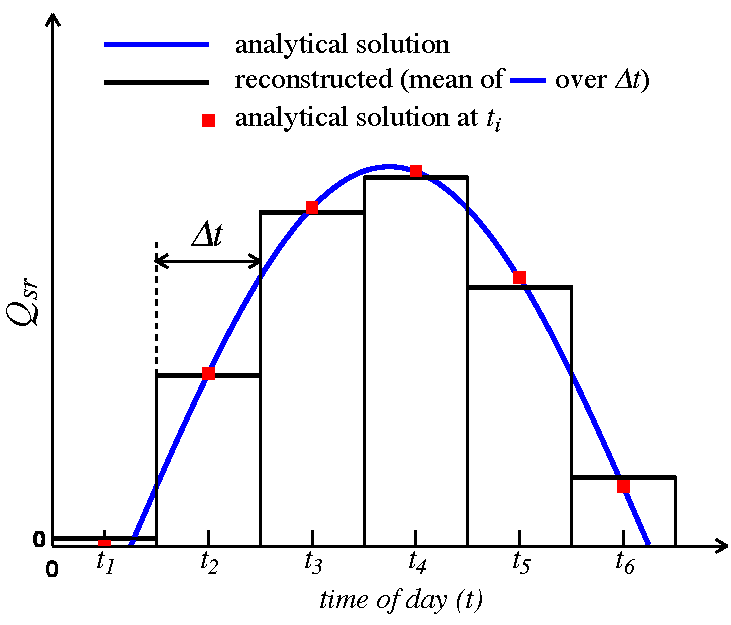
\includegraphics[width=0.8\textwidth]{Fig_SBC_diurnal}
\caption{ \protect\label{fig:SBC_diurnal}
  Example of recontruction of the diurnal cycle variation of short wave flux from daily mean values.
  The reconstructed diurnal cycle (black line) is chosen as
  the mean value of the analytical cycle (blue line) over a time step,
  not as the mid time step value of the analytically cycle (red square).
  From \citet{Bernie_al_CD07}.}
\end{center}   \end{figure}
%>>>>>>>>>>>>>>>>>>>>>>>>>>>>

\cite{Bernie_al_JC05} have shown that to capture 90$\%$ of the diurnal variability of SST requires a vertical resolution in upper ocean of 1~m or better and a temporal resolution of the surface fluxes of 3~h or less.
Unfortunately high frequency forcing fields are rare, not to say inexistent.
Nevertheless, it is possible to obtain a reasonable diurnal cycle of the SST knowning only short wave flux (SWF) at
high frequency \citep{Bernie_al_CD07}.
Furthermore, only the knowledge of daily mean value of SWF is needed,
as higher frequency variations can be reconstructed from them,
assuming that the diurnal cycle of SWF is a scaling of the top of the atmosphere diurnal cycle of incident SWF.
The \cite{Bernie_al_CD07} reconstruction algorithm is available in \NEMO by
setting \np{ln\_dm2dc}\forcode{ = .true.} (a \textit{\ngn{namsbc}} namelist variable) when
using CORE bulk formulea (\np{ln\_blk\_core}\forcode{ = .true.}) or
the flux formulation (\np{ln\_flx}\forcode{ = .true.}).
The reconstruction is performed in the \mdl{sbcdcy} module.
The detail of the algoritm used can be found in the appendix~A of \cite{Bernie_al_CD07}.
The algorithm preserve the daily mean incoming SWF as the reconstructed SWF at
a given time step is the mean value of the analytical cycle over this time step (\autoref{fig:SBC_diurnal}).
The use of diurnal cycle reconstruction requires the input SWF to be daily
($i.e.$ a frequency of 24 and a time interpolation set to true in \np{sn\_qsr} namelist parameter).
Furthermore, it is recommended to have a least 8 surface module time step per day,
that is  $\rdt \ nn\_fsbc < 10,800~s = 3~h$.
An example of recontructed SWF is given in \autoref{fig:SBC_dcy} for a 12 reconstructed diurnal cycle,
one every 2~hours (from 1am to 11pm).

%>>>>>>>>>>>>>>>>>>>>>>>>>>>>
\begin{figure}[!t]  \begin{center}
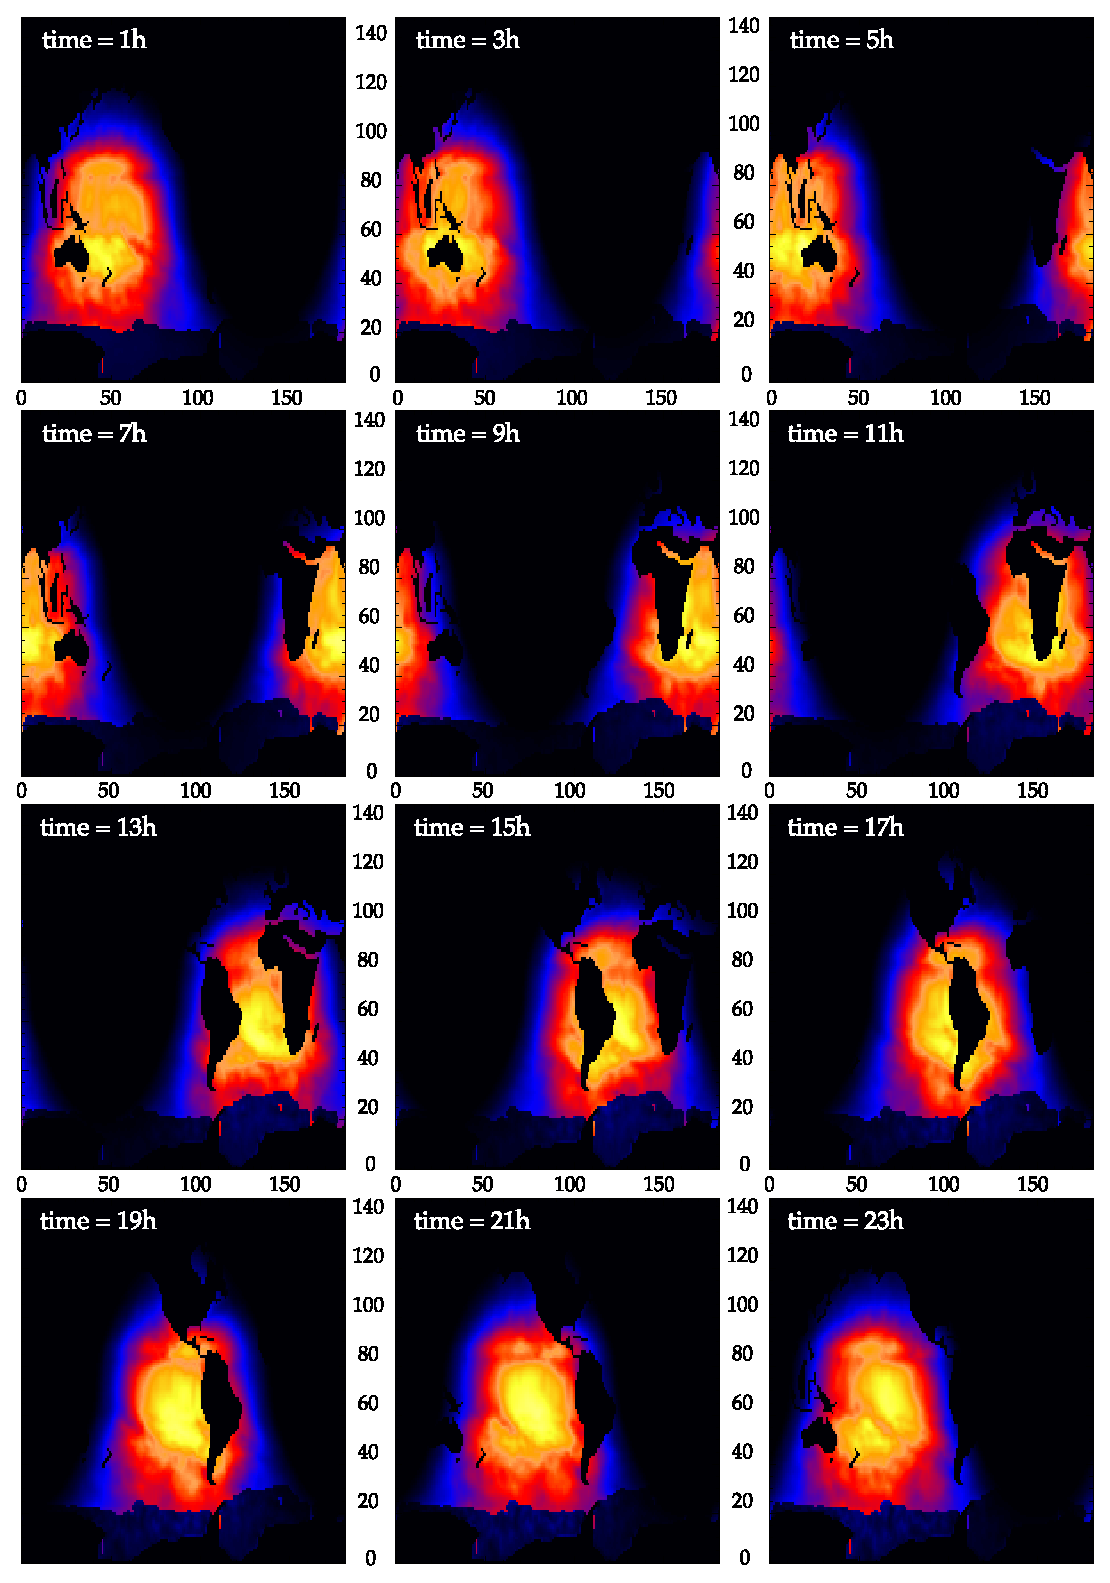
\includegraphics[width=0.7\textwidth]{Fig_SBC_dcy}
\caption{ \protect\label{fig:SBC_dcy}
  Example of recontruction of the diurnal cycle variation of short wave flux from
  daily mean values on an ORCA2 grid with a time sampling of 2~hours (from 1am to 11pm).
  The display is on (i,j) plane. }
\end{center}   \end{figure}
%>>>>>>>>>>>>>>>>>>>>>>>>>>>>

Note also that the setting a diurnal cycle in SWF is highly recommended when
the top layer thickness approach 1~m or less, otherwise large error in SST can appear due to
an inconsistency between the scale of the vertical resolution and the forcing acting on that scale.

% -------------------------------------------------------------------------------------------------------------
%        Rotation of vector pairs onto the model grid directions
% -------------------------------------------------------------------------------------------------------------
\subsection{Rotation of vector pairs onto the model grid directions}
\label{subsec:SBC_rotation}

When using a flux (\np{ln\_flx}\forcode{ = .true.}) or
bulk (\np{ln\_clio}\forcode{ = .true.} or \np{ln\_core}\forcode{ = .true.}) formulation,
pairs of vector components can be rotated from east-north directions onto the local grid directions.
This is particularly useful when interpolation on the fly is used since here any vectors are likely to
be defined relative to a rectilinear grid.
To activate this option a non-empty string is supplied in the rotation pair column of the relevant namelist.
The eastward component must start with "U" and the northward component with "V".  
The remaining characters in the strings are used to identify which pair of components go together.
So for example, strings "U1" and "V1" next to "utau" and "vtau" would pair the wind stress components together and
rotate them on to the model grid directions;
"U2" and "V2" could be used against a second pair of components, and so on.
The extra characters used in the strings are arbitrary.
The rot\_rep routine from the \mdl{geo2ocean} module is used to perform the rotation.

% -------------------------------------------------------------------------------------------------------------
%        Surface restoring to observed SST and/or SSS
% -------------------------------------------------------------------------------------------------------------
\subsection{Surface restoring to observed SST and/or SSS (\protect\mdl{sbcssr})}
\label{subsec:SBC_ssr}
%------------------------------------------namsbc_ssr----------------------------------------------------

\nlst{namsbc_ssr} 
%-------------------------------------------------------------------------------------------------------------

IOptions are defined through the \ngn{namsbc\_ssr} namelist variables.
On forced mode using a flux formulation (\np{ln\_flx}\forcode{ = .true.}),
a feedback term \emph{must} be added to the surface heat flux $Q_{ns}^o$:
\begin{equation} \label{eq:sbc_dmp_q}
Q_{ns} = Q_{ns}^o + \frac{dQ}{dT} \left( \left. T \right|_{k=1} - SST_{Obs} \right)
\end{equation}
where SST is a sea surface temperature field (observed or climatological),
$T$ is the model surface layer temperature and
$\frac{dQ}{dT}$ is a negative feedback coefficient usually taken equal to $-40~W/m^2/K$.
For a $50~m$ mixed-layer depth, this value corresponds to a relaxation time scale of two months. 
This term ensures that if $T$ perfectly matches the supplied SST, then $Q$ is equal to $Q_o$. 

In the fresh water budget, a feedback term can also be added.
Converted into an equivalent freshwater flux, it takes the following expression :

\begin{equation} \label{eq:sbc_dmp_emp}
\textit{emp} = \textit{emp}_o + \gamma_s^{-1} e_{3t}  \frac{  \left(\left.S\right|_{k=1}-SSS_{Obs}\right)}
												         {\left.S\right|_{k=1}}
\end{equation}

where $\textit{emp}_{o }$ is a net surface fresh water flux
(observed, climatological or an atmospheric model product),
\textit{SSS}$_{Obs}$ is a sea surface salinity
(usually a time interpolation of the monthly mean Polar Hydrographic Climatology \citep{Steele2001}),
$\left.S\right|_{k=1}$ is the model surface layer salinity and
$\gamma_s$ is a negative feedback coefficient which is provided as a namelist parameter.
Unlike heat flux, there is no physical justification for the feedback term in \autoref{eq:sbc_dmp_emp} as
the atmosphere does not care about ocean surface salinity \citep{Madec1997}.
The SSS restoring term should be viewed as a flux correction on freshwater fluxes to
reduce the uncertainties we have on the observed freshwater budget.

% -------------------------------------------------------------------------------------------------------------
%        Handling of ice-covered area
% -------------------------------------------------------------------------------------------------------------
\subsection{Handling of ice-covered area  (\textit{sbcice\_...})}
\label{subsec:SBC_ice-cover}

The presence at the sea surface of an ice covered area modifies all the fluxes transmitted to the ocean.
There are several way to handle sea-ice in the system depending on
the value of the \np{nn\_ice} namelist parameter found in \ngn{namsbc} namelist.
\begin{description}
\item[nn{\_}ice = 0]
  there will never be sea-ice in the computational domain.
  This is a typical namelist value used for tropical ocean domain.
  The surface fluxes are simply specified for an ice-free ocean.
  No specific things is done for sea-ice.
\item[nn{\_}ice = 1]
  sea-ice can exist in the computational domain, but no sea-ice model is used.
  An observed ice covered area is read in a file.
  Below this area, the SST is restored to the freezing point and
  the heat fluxes are set to $-4~W/m^2$ ($-2~W/m^2$) in the northern (southern) hemisphere.
  The associated modification of the freshwater fluxes are done in such a way that
  the change in buoyancy fluxes remains zero.
  This prevents deep convection to occur when trying to reach the freezing point
  (and so ice covered area condition) while the SSS is too large.
  This manner of managing sea-ice area, just by using si IF case,
  is usually referred as the \textit{ice-if} model.
  It can be found in the \mdl{sbcice{\_}if} module.
\item[nn{\_}ice = 2 or more]
  A full sea ice model is used.
  This model computes the ice-ocean fluxes,
  that are combined with the air-sea fluxes using the ice fraction of each model cell to
  provide the surface ocean fluxes.
  Note that the activation of a sea-ice model is is done by defining a CPP key (\key{lim3} or \key{cice}).
  The activation automatically overwrites the read value of nn{\_}ice to its appropriate value
  ($i.e.$ $2$ for LIM-3 or $3$ for CICE).
\end{description}

% {Description of Ice-ocean interface to be added here or in LIM 2 and 3 doc ?}

\subsection{Interface to CICE (\protect\mdl{sbcice\_cice})}
\label{subsec:SBC_cice}

It is now possible to couple a regional or global NEMO configuration (without AGRIF)
to the CICE sea-ice model by using \key{cice}.
The CICE code can be obtained from \href{http://oceans11.lanl.gov/trac/CICE/}{LANL} and
the additional 'hadgem3' drivers will be required, even with the latest code release.
Input grid files consistent with those used in NEMO will also be needed,
and CICE CPP keys \textbf{ORCA\_GRID}, \textbf{CICE\_IN\_NEMO} and \textbf{coupled} should be used
(seek advice from UKMO if necessary).
Currently the code is only designed to work when using the CORE forcing option for NEMO
(with \textit{calc\_strair}\forcode{ = .true.} and \textit{calc\_Tsfc}\forcode{ = .true.} in the CICE name-list),
or alternatively when NEMO is coupled to the HadGAM3 atmosphere model
(with \textit{calc\_strair}\forcode{ = .false.} and \textit{calc\_Tsfc}\forcode{ = false}).
The code is intended to be used with \np{nn\_fsbc} set to 1
(although coupling ocean and ice less frequently should work,
it is possible the calculation of some of the ocean-ice fluxes needs to be modified slightly -
the user should check that results are not significantly different to the standard case).

There are two options for the technical coupling between NEMO and CICE.
The standard version allows complete flexibility for the domain decompositions in the individual models,
but this is at the expense of global gather and scatter operations in the coupling which
become very expensive on larger numbers of processors.
The alternative option (using \key{nemocice\_decomp} for both NEMO and CICE) ensures that
the domain decomposition is identical in both models (provided domain parameters are set appropriately,
and \textit{processor\_shape~=~square-ice} and \textit{distribution\_wght~=~block} in the CICE name-list) and
allows much more efficient direct coupling on individual processors.
This solution scales much better although it is at the expense of having more idle CICE processors in areas where
there is no sea ice.

% -------------------------------------------------------------------------------------------------------------
%        Freshwater budget control 
% -------------------------------------------------------------------------------------------------------------
\subsection{Freshwater budget control (\protect\mdl{sbcfwb})}
\label{subsec:SBC_fwb}

For global ocean simulation it can be useful to introduce a control of the mean sea level in order to
prevent unrealistic drift of the sea surface height due to inaccuracy in the freshwater fluxes.
In \NEMO, two way of controlling the the freshwater budget. 
\begin{description}
\item[\np{nn\_fwb}\forcode{ = 0}]
  no control at all.
  The mean sea level is free to drift, and will certainly do so.
\item[\np{nn\_fwb}\forcode{ = 1}]
  global mean \textit{emp} set to zero at each model time step. 
%Note that with a sea-ice model, this technique only control the mean sea level with linear free surface (\key{vvl} not defined) and no mass flux between ocean and ice (as it is implemented in the current ice-ocean coupling). 
\item[\np{nn\_fwb}\forcode{ = 2}]
  freshwater budget is adjusted from the previous year annual mean budget which
  is read in the \textit{EMPave\_old.dat} file.
  As the model uses the Boussinesq approximation, the annual mean fresh water budget is simply evaluated from
  the change in the mean sea level at January the first and saved in the \textit{EMPav.dat} file. 
\end{description}



% Griffies doc:
% When running ocean-ice simulations, we are not explicitly representing land processes, 
% such as rivers, catchment areas, snow accumulation, etc. However, to reduce model drift, 
% it is important to balance the hydrological cycle in ocean-ice models. 
% We thus need to prescribe some form of global normalization to the precipitation minus evaporation plus river runoff. 
% The result of the normalization should be a global integrated zero net water input to the ocean-ice system over 
% a chosen time scale. 
%How often the normalization is done is a matter of choice. In mom4p1, we choose to do so at each model time step, 
% so that there is always a zero net input of water to the ocean-ice system. 
% Others choose to normalize over an annual cycle, in which case the net imbalance over an annual cycle is used 
% to alter the subsequent year�s water budget in an attempt to damp the annual water imbalance. 
% Note that the annual budget approach may be inappropriate with interannually varying precipitation forcing. 
% When running ocean-ice coupled models, it is incorrect to include the water transport between the ocean 
% and ice models when aiming to balance the hydrological cycle. 
% The reason is that it is the sum of the water in the ocean plus ice that should be balanced when running ocean-ice models, 
% not the water in any one sub-component. As an extreme example to illustrate the issue, 
% consider an ocean-ice model with zero initial sea ice. As the ocean-ice model spins up, 
% there should be a net accumulation of water in the growing sea ice, and thus a net loss of water from the ocean. 
% The total water contained in the ocean plus ice system is constant, but there is an exchange of water between 
% the subcomponents. This exchange should not be part of the normalization used to balance the hydrological cycle 
% in ocean-ice models. 


\end{document}
